\documentclass{standalone}
\usepackage{tikz}
\usetikzlibrary{patterns, positioning}


\begin{document}
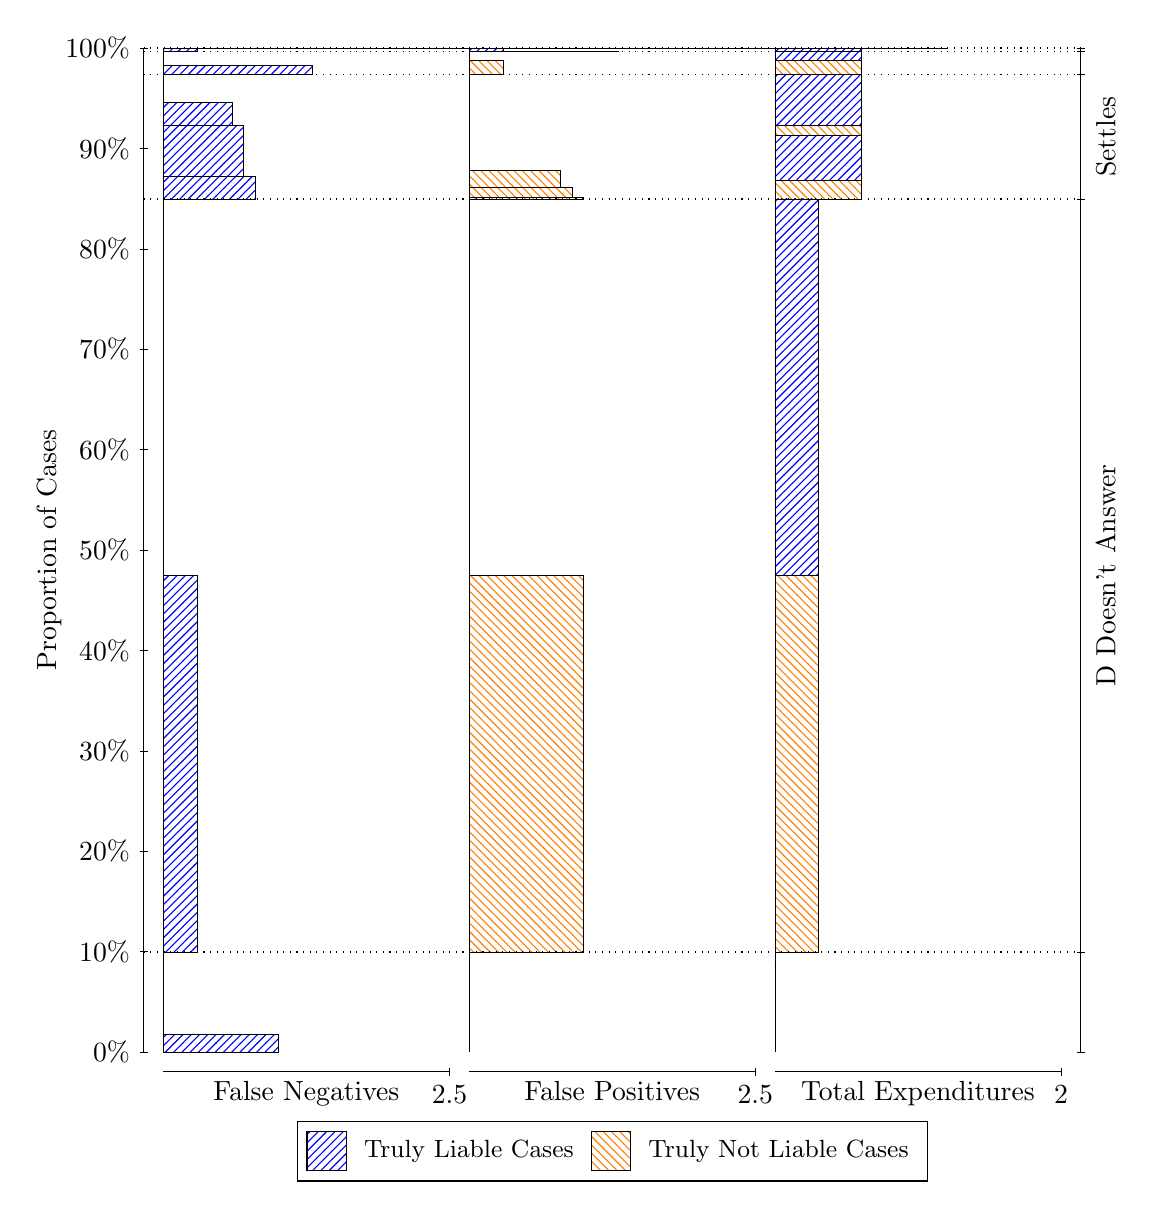
\begin{tikzpicture}
\draw[black, very thin] (1.5,1.75) -- (1.5,14.5);
\node[rotate=90, text=black, anchor=center] at (0.3, 8.125) {Proportion of Cases};
\draw[black, very thin] (1.45,1.75) -- (1.55,1.75);
\node[text=black, anchor=east] at (1.45, 1.75) {0\%};
\draw[black, very thin] (1.45,3.025) -- (1.55,3.025);
\node[text=black, anchor=east] at (1.45, 3.025) {10\%};
\draw[black, very thin] (1.45,4.3) -- (1.55,4.3);
\node[text=black, anchor=east] at (1.45, 4.3) {20\%};
\draw[black, very thin] (1.45,5.575) -- (1.55,5.575);
\node[text=black, anchor=east] at (1.45, 5.575) {30\%};
\draw[black, very thin] (1.45,6.85) -- (1.55,6.85);
\node[text=black, anchor=east] at (1.45, 6.85) {40\%};
\draw[black, very thin] (1.45,8.125) -- (1.55,8.125);
\node[text=black, anchor=east] at (1.45, 8.125) {50\%};
\draw[black, very thin] (1.45,9.4) -- (1.55,9.4);
\node[text=black, anchor=east] at (1.45, 9.4) {60\%};
\draw[black, very thin] (1.45,10.675) -- (1.55,10.675);
\node[text=black, anchor=east] at (1.45, 10.675) {70\%};
\draw[black, very thin] (1.45,11.95) -- (1.55,11.95);
\node[text=black, anchor=east] at (1.45, 11.95) {80\%};
\draw[black, very thin] (1.45,13.225) -- (1.55,13.225);
\node[text=black, anchor=east] at (1.45, 13.225) {90\%};
\draw[black, very thin] (1.45,14.5) -- (1.55,14.5);
\node[text=black, anchor=east] at (1.45, 14.5) {100\%};

\draw[black, very thin] (13.4,1.75) -- (13.4,14.5);
\draw[black, very thin] (13.35,1.75) -- (13.45,1.75);
\node[anchor=west] at (13.35, 1.75) {};
\draw[black, very thin] (13.35,3.0201) -- (13.45,3.0201);
\node[anchor=west] at (13.35, 3.0201) {};
\draw[black, very thin] (13.35,12.583) -- (13.45,12.583);
\node[anchor=west] at (13.35, 12.583) {};
\draw[black, very thin] (13.35,14.168) -- (13.45,14.168);
\node[anchor=west] at (13.35, 14.168) {};
\draw[black, very thin] (13.35,14.454) -- (13.45,14.454);
\node[anchor=west] at (13.35, 14.454) {};
\draw[black, very thin] (13.35,14.5) -- (13.45,14.5);
\node[anchor=west] at (13.35, 14.5) {};
\draw[black, very thin] (13.35,14.5) -- (13.45,14.5);
\node[anchor=west] at (13.35, 14.5) {};
\draw[black, very thin] (13.35,14.5) -- (13.45,14.5);
\node[anchor=west] at (13.35, 14.5) {};

\draw[black, very thin, pattern color=blue, pattern=north east lines] (1.75,1.75) rectangle (3.2033,1.9686);
\draw[black, very thin, pattern color=orange, pattern=north west lines] (1.75,1.9686) rectangle (1.75,3.0201);
\draw[black, very thin, pattern color=blue, pattern=north east lines] (1.75,3.0201) rectangle (2.186,7.8013);
\draw[black, very thin, pattern color=orange, pattern=north west lines] (1.75,7.8013) rectangle (1.75,12.583);
\draw[black, very thin, pattern color=blue, pattern=north east lines] (1.75,12.583) rectangle (2.9127,12.872);
\draw[black, very thin, pattern color=blue, pattern=north east lines] (1.75,12.872) rectangle (2.7673,13.521);
\draw[black, very thin, pattern color=blue, pattern=north east lines] (1.75,13.521) rectangle (2.622,13.808);
\draw[black, very thin, pattern color=orange, pattern=north west lines] (1.75,13.808) rectangle (1.75,14.168);
\draw[black, very thin, pattern color=blue, pattern=north east lines] (1.75,14.168) rectangle (3.6393,14.279);
\draw[black, very thin, pattern color=orange, pattern=north west lines] (1.75,14.279) rectangle (1.75,14.454);
\draw[black, very thin, pattern color=blue, pattern=north east lines] (1.75,14.454) rectangle (2.186,14.492);
\draw[black, very thin, pattern color=orange, pattern=north west lines] (1.75,14.492) rectangle (1.75,14.5);
\draw[black, very thin, pattern color=blue, pattern=north east lines] (1.75,14.5) rectangle (5.8193,14.5);
\draw[black, very thin, pattern color=orange, pattern=north west lines] (1.75,14.5) rectangle (1.75,14.5);
\draw[black, very thin, pattern color=orange, pattern=north west lines] (1.75,14.5) rectangle (1.75,14.5);
\draw[black, very thin, pattern color=blue, pattern=north east lines] (1.75,14.5) rectangle (1.75,14.5);
\draw[black, very thin, pattern color=orange, pattern=north west lines] (5.6333,1.75) rectangle (5.6333,2.8015);
\draw[black, very thin, pattern color=blue, pattern=north east lines] (5.6333,2.8015) rectangle (5.6333,3.0201);
\draw[black, very thin, pattern color=orange, pattern=north west lines] (5.6333,3.0201) rectangle (7.0867,7.8014);
\draw[black, very thin, pattern color=blue, pattern=north east lines] (5.6333,7.8014) rectangle (5.6333,12.583);
\draw[black, very thin, pattern color=orange, pattern=north west lines] (5.6333,12.583) rectangle (7.0867,12.607);
\draw[black, very thin, pattern color=orange, pattern=north west lines] (5.6333,12.607) rectangle (6.9413,12.729);
\draw[black, very thin, pattern color=orange, pattern=north west lines] (5.6333,12.729) rectangle (6.796,12.942);
\draw[black, very thin, pattern color=blue, pattern=north east lines] (5.6333,12.942) rectangle (5.6333,14.168);
\draw[black, very thin, pattern color=orange, pattern=north west lines] (5.6333,14.168) rectangle (6.0693,14.343);
\draw[black, very thin, pattern color=blue, pattern=north east lines] (5.6333,14.343) rectangle (5.6333,14.454);
\draw[black, very thin, pattern color=orange, pattern=north west lines] (5.6333,14.454) rectangle (7.5227,14.462);
\draw[black, very thin, pattern color=blue, pattern=north east lines] (5.6333,14.462) rectangle (6.0693,14.5);
\draw[black, very thin, pattern color=orange, pattern=north west lines] (5.6333,14.5) rectangle (5.6333,14.5);
\draw[black, very thin, pattern color=blue, pattern=north east lines] (5.6333,14.5) rectangle (5.6333,14.5);
\draw[black, very thin, pattern color=orange, pattern=north west lines] (5.6333,14.5) rectangle (9.7027,14.5);
\draw[black, very thin, pattern color=blue, pattern=north east lines] (5.6333,14.5) rectangle (8.2493,14.5);
\draw[black, very thin, pattern color=orange, pattern=north west lines] (9.5167,1.75) rectangle (9.5167,2.8015);
\draw[black, very thin, pattern color=blue, pattern=north east lines] (9.5167,2.8015) rectangle (9.5167,3.0201);
\draw[black, very thin, pattern color=orange, pattern=north west lines] (9.5167,3.0201) rectangle (10.062,7.8014);
\draw[black, very thin, pattern color=blue, pattern=north east lines] (9.5167,7.8014) rectangle (10.062,12.583);
\draw[black, very thin, pattern color=orange, pattern=north west lines] (9.5167,12.583) rectangle (10.607,12.819);
\draw[black, very thin, pattern color=blue, pattern=north east lines] (9.5167,12.819) rectangle (10.607,13.395);
\draw[black, very thin, pattern color=orange, pattern=north west lines] (9.5167,13.395) rectangle (10.607,13.518);
\draw[black, very thin, pattern color=blue, pattern=north east lines] (9.5167,13.518) rectangle (10.607,14.168);
\draw[black, very thin, pattern color=orange, pattern=north west lines] (9.5167,14.168) rectangle (10.607,14.343);
\draw[black, very thin, pattern color=blue, pattern=north east lines] (9.5167,14.343) rectangle (10.607,14.454);
\draw[black, very thin, pattern color=orange, pattern=north west lines] (9.5167,14.454) rectangle (10.607,14.462);
\draw[black, very thin, pattern color=blue, pattern=north east lines] (9.5167,14.462) rectangle (10.607,14.5);
\draw[black, very thin, pattern color=orange, pattern=north west lines] (9.5167,14.5) rectangle (11.697,14.5);
\draw[black, very thin, pattern color=blue, pattern=north east lines] (9.5167,14.5) rectangle (11.697,14.5);
\draw[black, very thin, pattern color=orange, pattern=north west lines] (9.5167,14.5) rectangle (11.697,14.5);
\draw[black, very thin, pattern color=blue, pattern=north east lines] (9.5167,14.5) rectangle (11.697,14.5);
\draw[black, dotted] (1.5,3.0201) -- (13.4,3.0201);
\draw[black, dotted] (1.5,12.583) -- (13.4,12.583);
\draw[black, dotted] (1.5,14.168) -- (13.4,14.168);
\draw[black, dotted] (1.5,14.454) -- (13.4,14.454);
\draw[black, dotted] (1.5,14.5) -- (13.4,14.5);
\draw[black, dotted] (1.5,14.5) -- (13.4,14.5);
\draw[black, very thin] (1.75,1.5) -- (5.3833,1.5);
\node[text=black, anchor=north] at (3.5667, 1.5) {False Negatives};
\draw[black, very thin] (5.3833,1.45) -- (5.3833,1.55);
\node[text=black, anchor=north] at (5.3833, 1.45) {2.5};

\draw[black, very thin] (5.6333,1.5) -- (9.2667,1.5);
\node[text=black, anchor=north] at (7.45, 1.5) {False Positives};
\draw[black, very thin] (9.2667,1.45) -- (9.2667,1.55);
\node[text=black, anchor=north] at (9.2667, 1.45) {2.5};

\draw[black, very thin] (9.5167,1.5) -- (13.15,1.5);
\node[text=black, anchor=north] at (11.333, 1.5) {Total Expenditures};
\draw[black, very thin] (13.15,1.45) -- (13.15,1.55);
\node[text=black, anchor=north] at (13.15, 1.45) {2};


\node[text=black, centered, rotate=90] at (13.72, 7.8013) {D Doesn't Answer};
\node[text=black, centered, rotate=90] at (13.72, 13.375) {Settles};





\draw (7.449999999999999,1.5) node[draw=none] (baseCoordinate) {};
\begin{scope}[align=center]
        \matrix[scale=0.5, draw=black, below=0.5cm of baseCoordinate, nodes={draw}, column sep=0.1cm]{
            \node[rectangle, draw, minimum width=0.5cm, minimum height=0.5cm, pattern color=blue, pattern=north east lines] {}; &
            \node[draw=none, font=\small, text=black] (B) {Truly Liable Cases}; &
            \node[rectangle, draw, minimum width=0.5cm, minimum height=0.5cm, pattern color=orange, pattern=north west lines] {}; &
            \node[draw=none, font=\small, text=black] (B) {Truly Not Liable Cases}; \\
            };
\end{scope}

\end{tikzpicture}
\end{document}